% meta.concepts: 3D moment
% meta.tags: realistic
% acknowledge: Peter Seiler & Luke Melander graciously shared Spring 2019 course material
% source: 2019 P. Seiler AEM2011 HW 3

In HW2 you analyzed the cable tensions for a meteorological tower at the University of Minnesota Eolos Wind
Research Field Station. The field station also has a 2.5MW Clipper Liberty Wind Turbine. The nacelle of this
turbine is located at an elevation of 80m and the rotor radius is $R = 48m$. The power produced by a wind
turbine is given by $P = \frac{1}{2}\rho A v^3 C_p (W)$ where $\rho = 1.225 (kg/m3)$ is the density of air, $A = \pi R^2$ is the circular
area of the rotor plane ($m^2$), $v$ is the wind speed ($m/s$) and $C_p$ (unitless) is the efficiency of the wind turbine.
\begin{enumerate}
  \item What is $C_P$ if the turbine generates $P = 2.5MW$ of power when the wind speed is $v = 11 m/sec$?
  \item The diagram (right) shows a right-handed coordinate system attached to the rotor hub. The wind flowing
past the blades causes a force to be distributed along each blade. For Blade 1 the effect is equivalent to a
single force F acting vertically at mid span ($x = 24m$). Assume a similar force acts perpendicular to the
other blades at midspan. What is the total moment about the center of the rotor hub, denoted $M_{hub}$, in
terms of this force $F$?
  \item The blades rotate at approximately $\omega = 1.6 rad/s$ about the horizontal rotor axis (z-axis). The power 
captured by a wind turbine can also be calculated as $P = M_{hub} \omega$. What is the effective force $F$ on each
blade if the turbine is producing $2.5 MW$ of power?
  \item Suppose you plan to design a turbine to operate off-shore where the wind speed will be $v = 22 m/sec$.
Assume this new turbine has the same efficiency $C_P$ (calculated in part $A$), rotational speed $\omega$ and radius
$R$ as the old turbine. You may also assume that the air density will remain the same. What is the power
generated by this new off-shore turbine? What is the effective force on the blades of this new turbine?
What is the impact on the design of the new turbine blades?
\end{enumerate}


\begin{figure}[ht!]
  \centering
  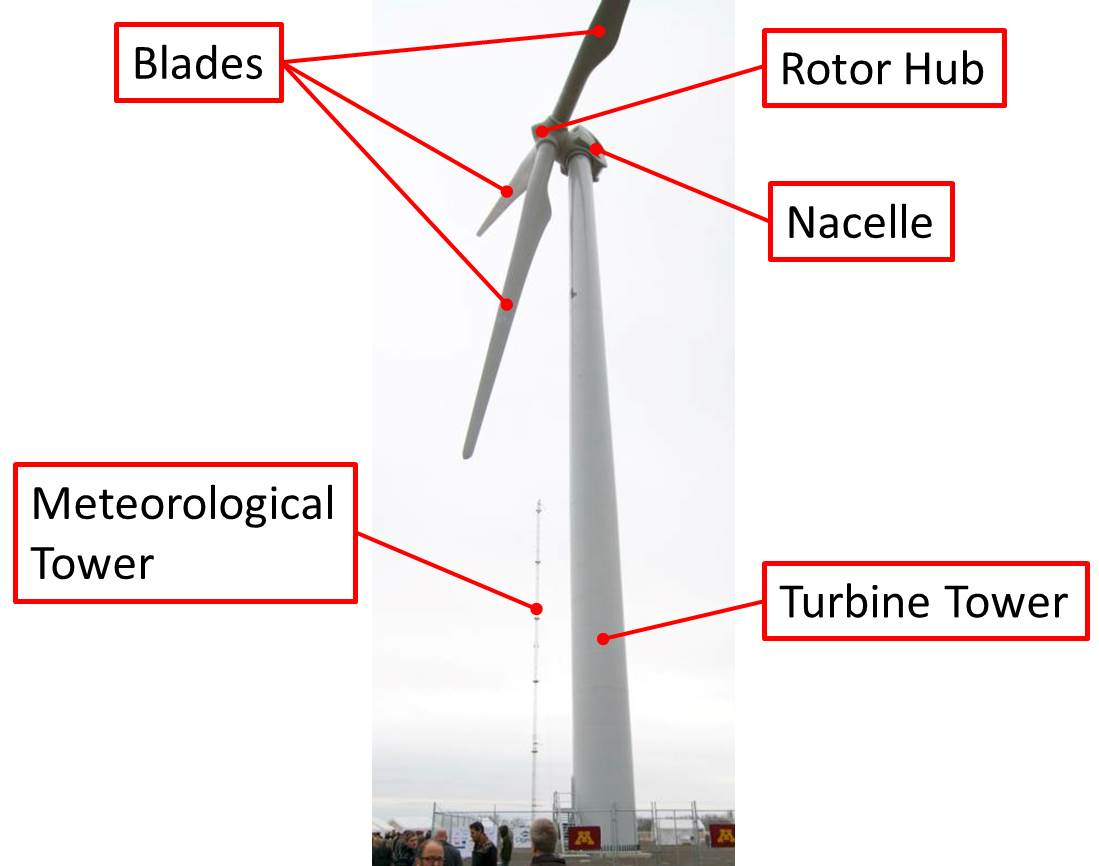
\includegraphics[height=1.8in]{figa.png}
  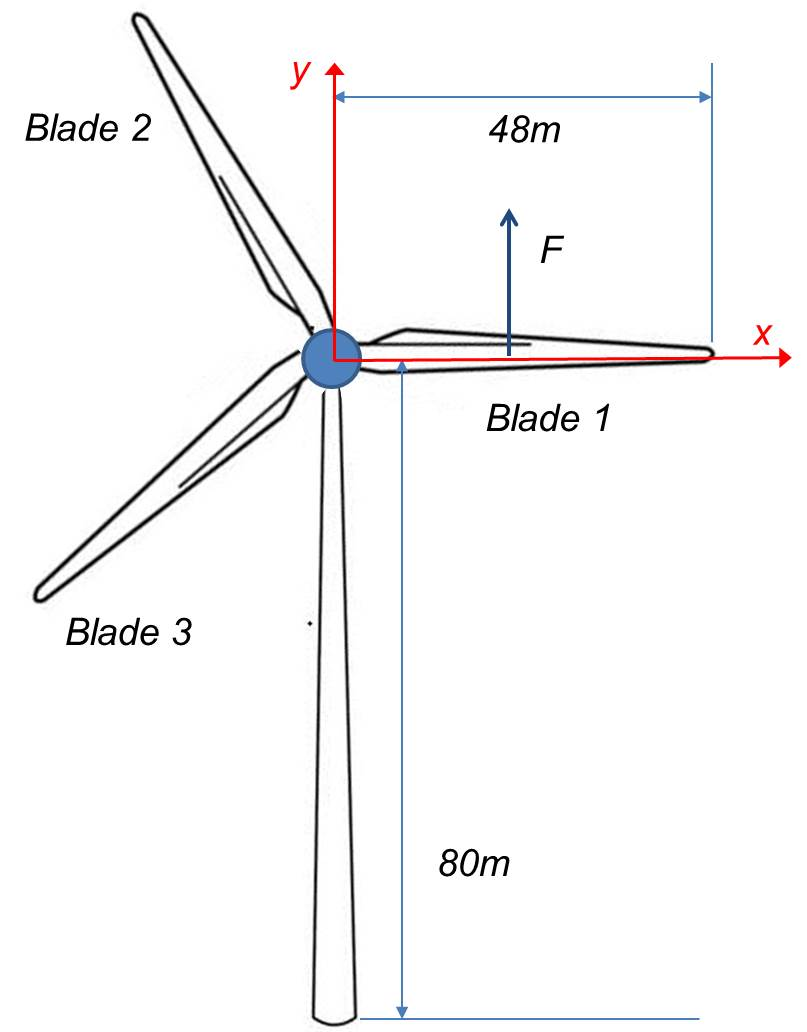
\includegraphics[height=1.8in]{figb.png}
  \caption*{Left: Clipper Liberty Turbine, Right: Diagram of turbine rotor}
\end{figure}

\iftoggle{flagSoln}{%
\vspace{.5cm}
\rule{\textwidth}{.4pt}
\vspace{.5cm}
\textbf{Solution:}
\begin{figure}[ht!]
  \centering
  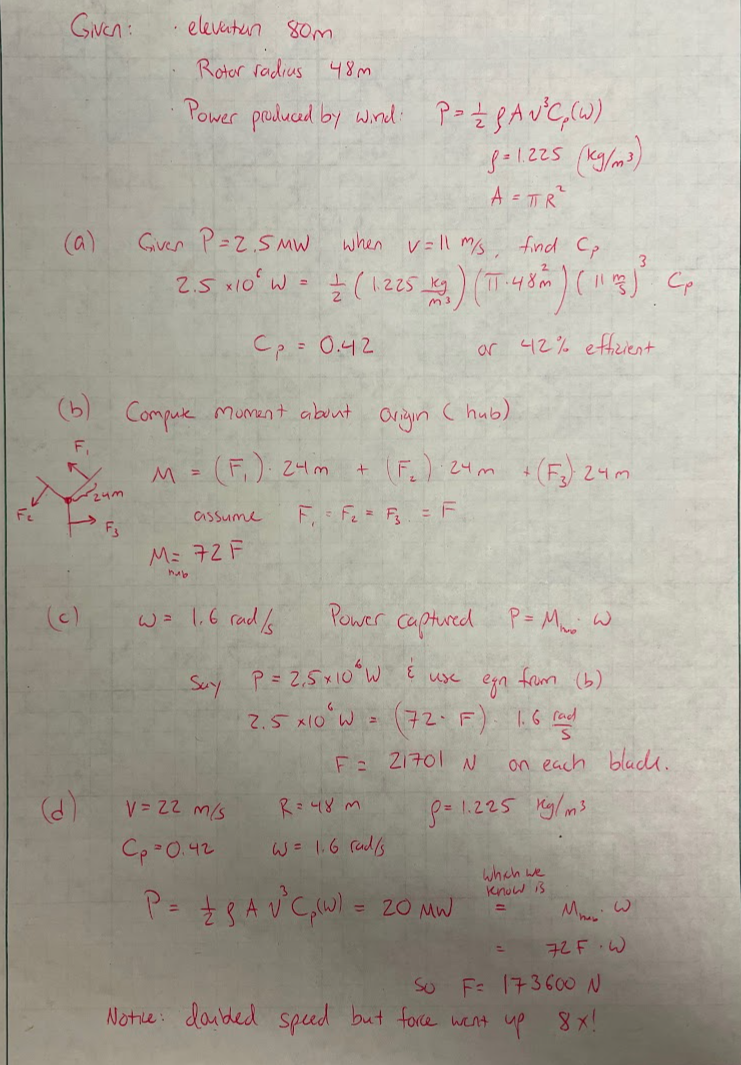
\includegraphics[width=0.9\textwidth,
	           height=0.3\textheight,
		   keepaspectratio]{soln.png}
\end{figure}
}{%
}%
